\documentclass[11pt]{article}
\usepackage[utf8]{inputenc}	% Para caracteres en español
\usepackage{amsmath,amsthm,amsfonts,amssymb,amscd}
\usepackage{multirow,booktabs}
\usepackage[table]{xcolor}
\usepackage{fullpage}
\usepackage{lastpage}
\usepackage{enumitem}
\usepackage{fancyhdr}
\usepackage{mathrsfs}
\usepackage{wrapfig}
\usepackage{setspace}
\usepackage{calc}
\usepackage{multicol}
\usepackage{cancel}
\usepackage[retainorgcmds]{IEEEtrantools}
\usepackage[margin=1cm]{geometry}
\usepackage{amsmath}
\newlength{\tabcont}
\setlength{\parindent}{0.0in}
\setlength{\parskip}{0.05in}
\usepackage{empheq}
\usepackage{framed}
\usepackage[most]{tcolorbox}
\usepackage{xcolor}
\usepackage{graphicx}
\usepackage{listings}
% -- Basic formatting
\usepackage[utf8]{inputenc}
\usepackage[english]{babel}
\usepackage{times}
\usepackage{caption}
\usepackage{subcaption}
\usepackage{placeins}
\setlength{\parindent}{0pt}
\usepackage{indentfirst}% -- Defining colors:
\usepackage[dvipsnames]{xcolor}
\definecolor{codegreen}{rgb}{0,0.6,0}
\definecolor{codegray}{rgb}{0.5,0.5,0.5}
\definecolor{codepurple}{rgb}{0.58,0,0.82}
\definecolor{backcolour}{rgb}{0.95,0.95,0.92}% Definig a custom style:
\lstdefinestyle{mystyle}{
    backgroundcolor=\color{backcolour},   
    commentstyle=\color{codepurple},
    keywordstyle=\color{NavyBlue},
    numberstyle=\tiny\color{codegray},
    stringstyle=\color{codepurple},
    basicstyle=\ttfamily\footnotesize\bfseries,
    breakatwhitespace=false,         
    breaklines=true,                 
    captionpos=t,                    
    keepspaces=true,                 
    numbers=left,                    
    numbersep=5pt,                  
    showspaces=false,                
    showstringspaces=false,
    showtabs=false,                  
    tabsize=2
}% -- Setting up the custom style:
\lstset{style=mystyle}
\lstset{
  style=mystyle,
  framexleftmargin=3.5mm,
  rulesepcolor=\color{black},
  linewidth=0.6\linewidth,
  xleftmargin=12pt,
  aboveskip=12pt,
  belowskip=12pt
}
\colorlet{shadecolor}{orange!15}
\parindent 0in
\parskip 1pt
\geometry{margin=1in, headsep=0.25in}
\theoremstyle{definition}
\newtheorem{defn}{Definition}
\newtheorem{reg}{Rule}
\newtheorem{exer}{Exercise}
\newtheorem{note}{Note}
\graphicspath{ {./images/} }
\linespread{0.75}
\begin{document}
\setcounter{section}{0}
\title{MIE223 Lecture Notes}

\thispagestyle{empty}

\begin{center}
{\LARGE \bf Time Series Data}\\
{\large MIE223}\\
Winter 2025
\end{center}
\section{Time Series Analysis}
\subsection{Time Series Data}
\begin{itemize}
  \item Time series data are
  \begin{itemize}
    \item Observations or measurements that
    are indexed according to time
    \item Instead of Xi we have Xt where t is
    specifically a time index  
  \end{itemize}
  \item Why does time make it different?
  \begin{itemize}
    \item The time index t has a special ordering  
    \item Data measured over time are not
    exchangeable, which is what we often
    assume when data are indexed by i
  \end{itemize}
\end{itemize}
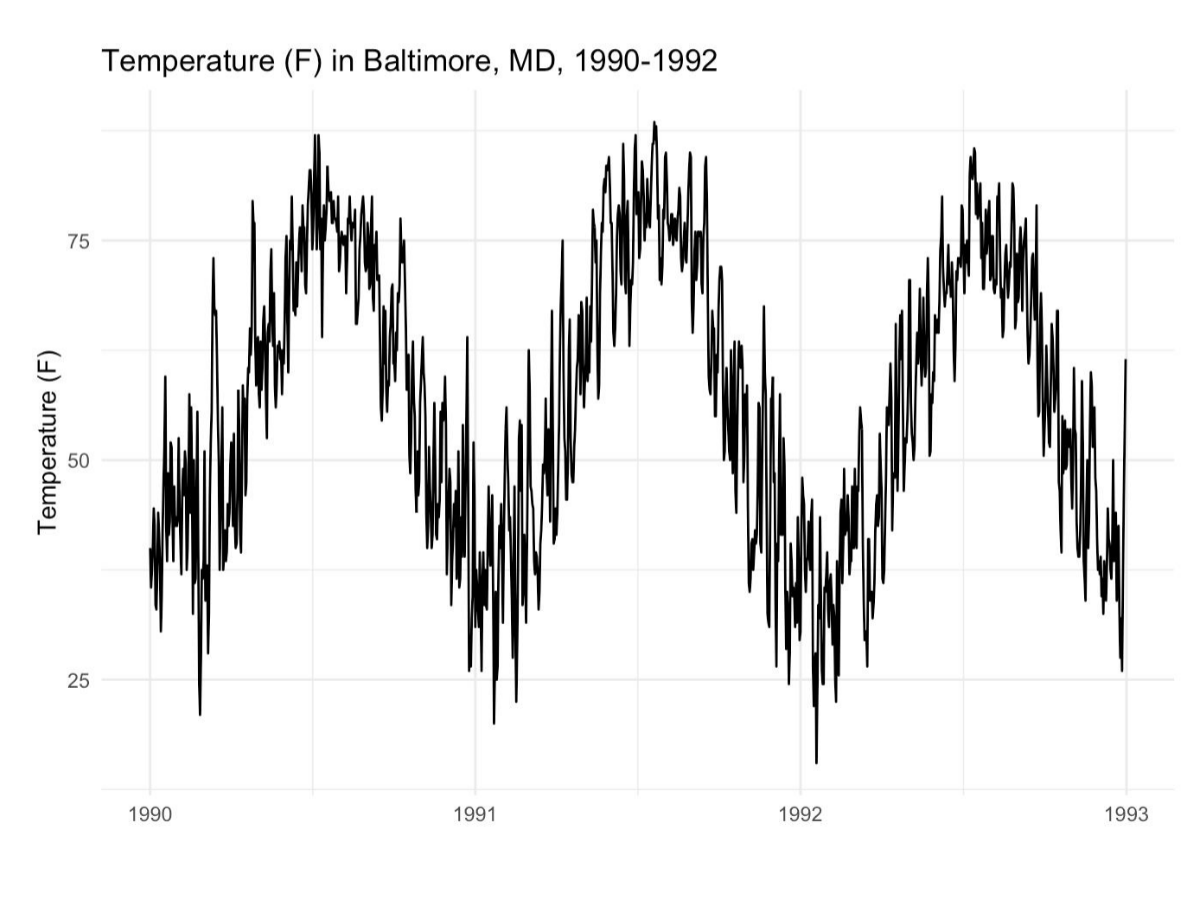
\includegraphics[width=\textwidth/2]{1.png}

\subsection{Goals of Time Series Analysis}
\begin{enumerate}
  \item Time Scale Analysis: at what scale is data useful to analyze?
  \begin{itemize}
    \item Is weather useful to analyze at the second, hour, or year level? Is it seasonal?
  \end{itemize}
  \item Smoothing: infer true state of past given a noisy signal (averaging out nearby timepoints)
  \begin{itemize}
    \item Assuming gradual change, use nearby values in a time series to smooth noise
  \end{itemize}
  \item Filtering: what is the true present state given a noisy signal
  \begin{itemize}
    \item Tracking a rocket trajectory
    \item Kalman filtering!
  \end{itemize}
  \item Forecasting: predict future values
  \begin{itemize}
    \item What will the stock price be tomorrow, given the past?
  \end{itemize}
  \item Regression: give time two series, can we predict the association between them?
  \begin{itemize}
    \item Does public sentiment predict the stock market at a delay?
  \end{itemize}
\end{enumerate}

\begin{note}
  Smoothing is about the past, filtering is about the present, forecasting is about the future
\end{note}

\section{Time Scale Analysis}
\subsection{Time Scale Analysis}
\begin{itemize}
  \item What time scales of variation dominate or account for the
  majority of temporal variation in the data? seasonal
  \item Is there a strong seasonal cycle in the observations of
  temperature in Baltimore, MD? Hope so
  \item Is the association between ambient air pollution and mortality in
  a city primarily driven by large annual changes in pollution
  levels or by short-term spikes? there can be multiple causes of mortality, and need longer timeframe
\end{itemize}
\begin{note}
  granger causality says that you can predict something if you know the past
\end{note}

\subsection{Trend-Season-Residual Decomposition}
A common tool to use is to
decompose a time series into

\begin{enumerate}
  \item Smooth long-term trend (trend)
  \item Seasonal variation (seasonal)
  \item Residual variation (day to day)
\end{enumerate}

The primary benefit is of
looking at long-term trend
and seasonal variation is that
they are highly interpretable
and are very common.

These graphs can be made by smoothing over different intervals.

\begin{itemize}
  \item Residual after subtracting
  long-term and seasonal trends
  \item Subtract long-term trend,
  smooth over local time window
  \item Smooth (average) over
  wide time window
\end{itemize}

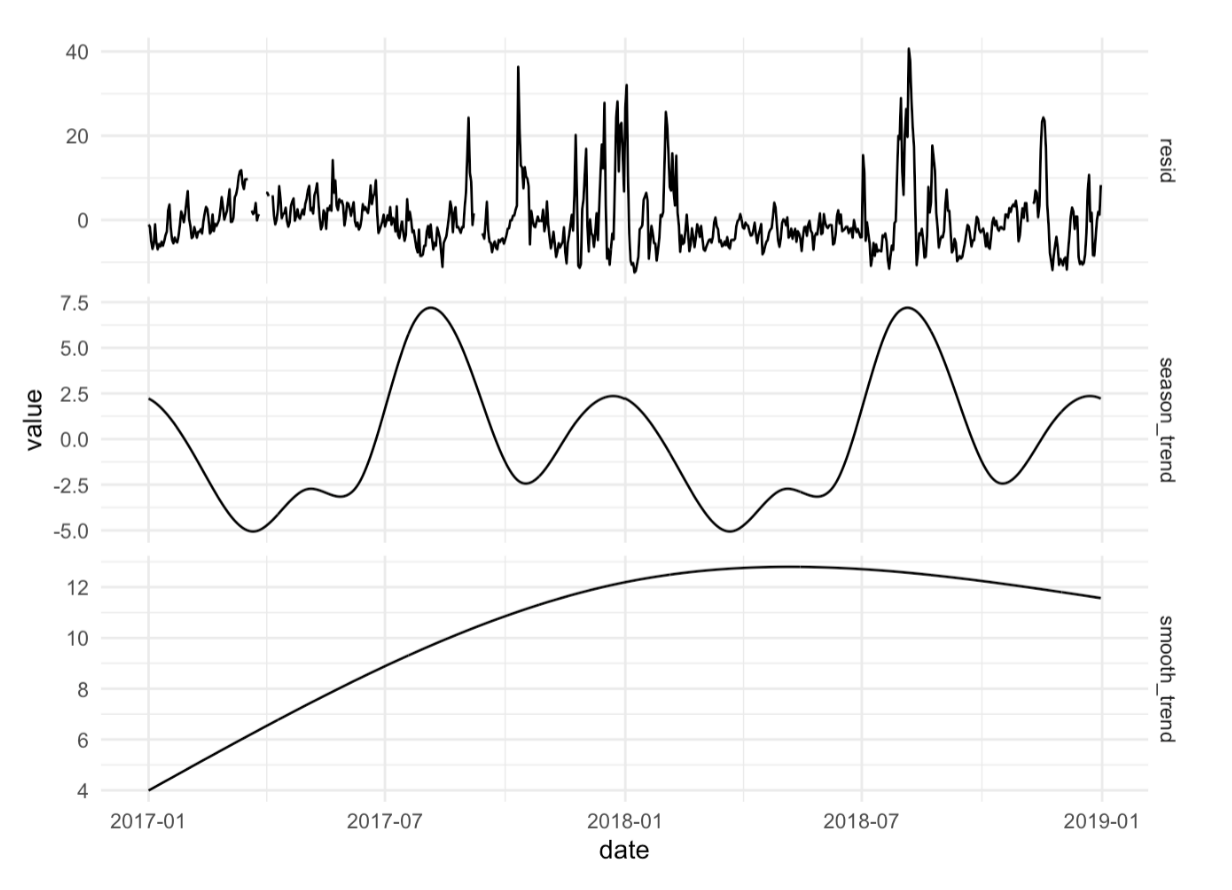
\includegraphics[width=\textwidth/2]{2.png}

\section{Time Series Regression with
Autocorrelation and
Cross-correlation}
\subsection{Regression (in general)}
Given a time series of two phenomena, what is the association
between them?

\begin{itemize}
  \item What is the association between daily levels of air pollution and daily
  values of cardiac hospitalizations?
  \item What is the lag (in months) between a change in a country’s
  unemployment rate and a change in the gross domestic product?
  \item What is the cumulative number of excess deaths that occurs in the 2
  weeks following a major hurricane?
\end{itemize}

\subsection{Recap of Covariance}
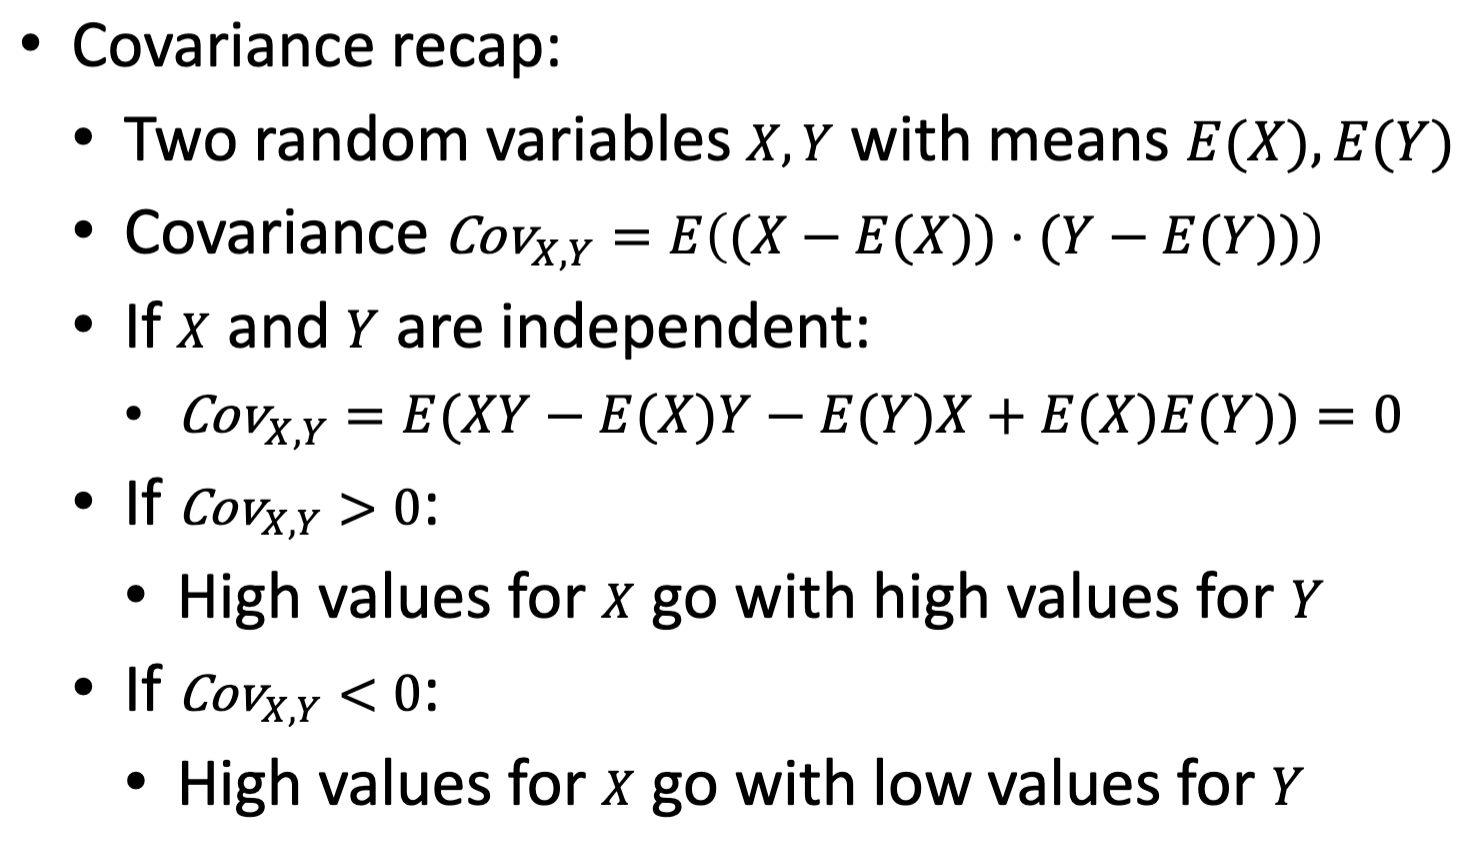
\includegraphics[width=\textwidth/2]{5.png}

probability is model based, stats is data based.

\begin{equation}
  E[XY] = E[X]E[Y] \text{if X and Y are independent}
\end{equation}

\subsection{Pearson Correlation Coefficient}
Covariance depends on the units in which X and Y are given

Therefore, we look at the Pearson correlation coefficient

If x and y have standard deviations $\sigma x$ and $\sigma y$ respectively:

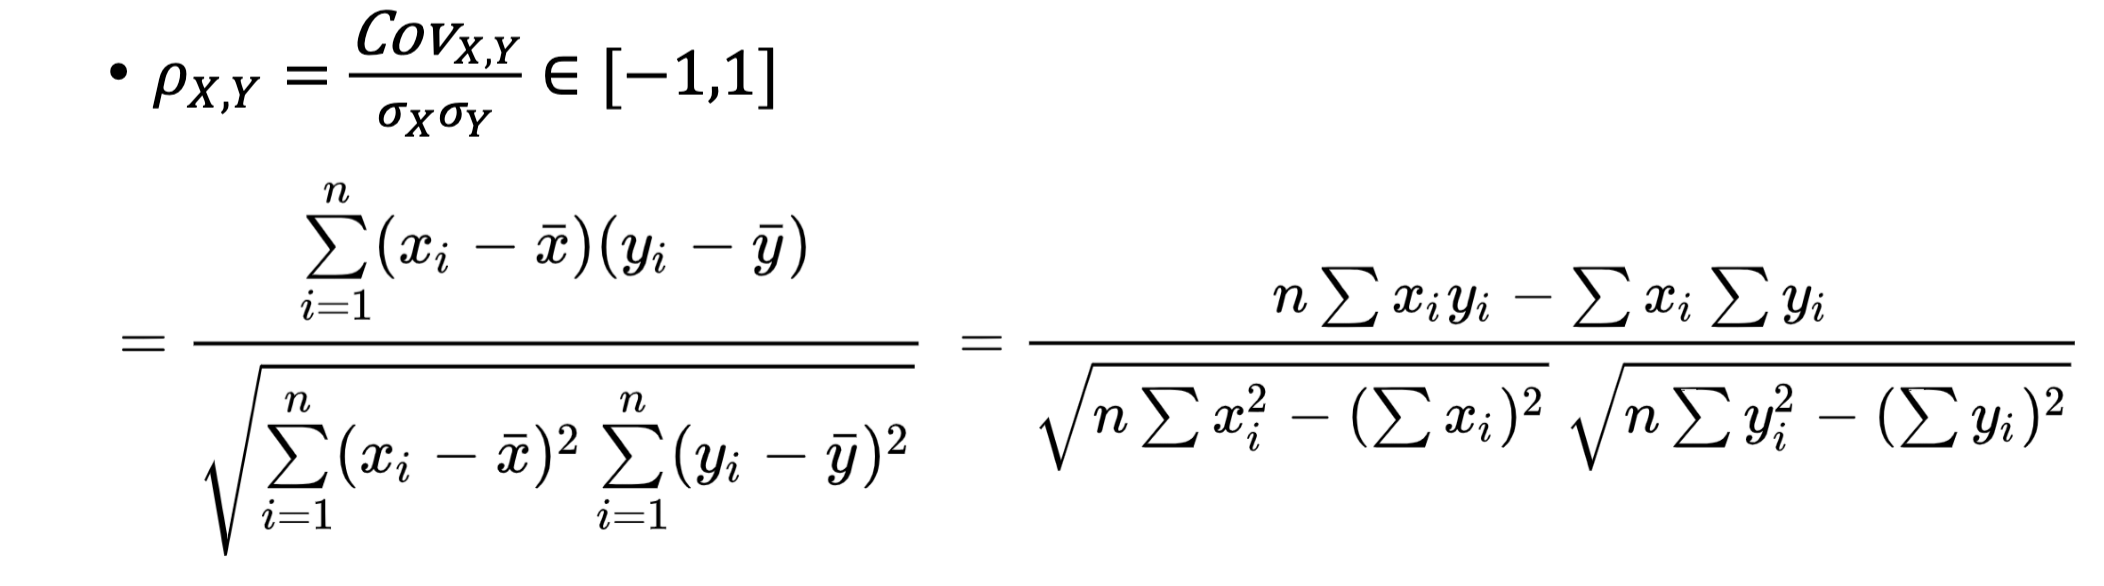
\includegraphics[width=\textwidth/2]{6.png}

independence implies correlation should be 0 but not vice versa

\subsection{Autocorrelation}
\textbf{Auto-correlation: Compare the correlation of a time series with itself
moved (lagged) by k positions}

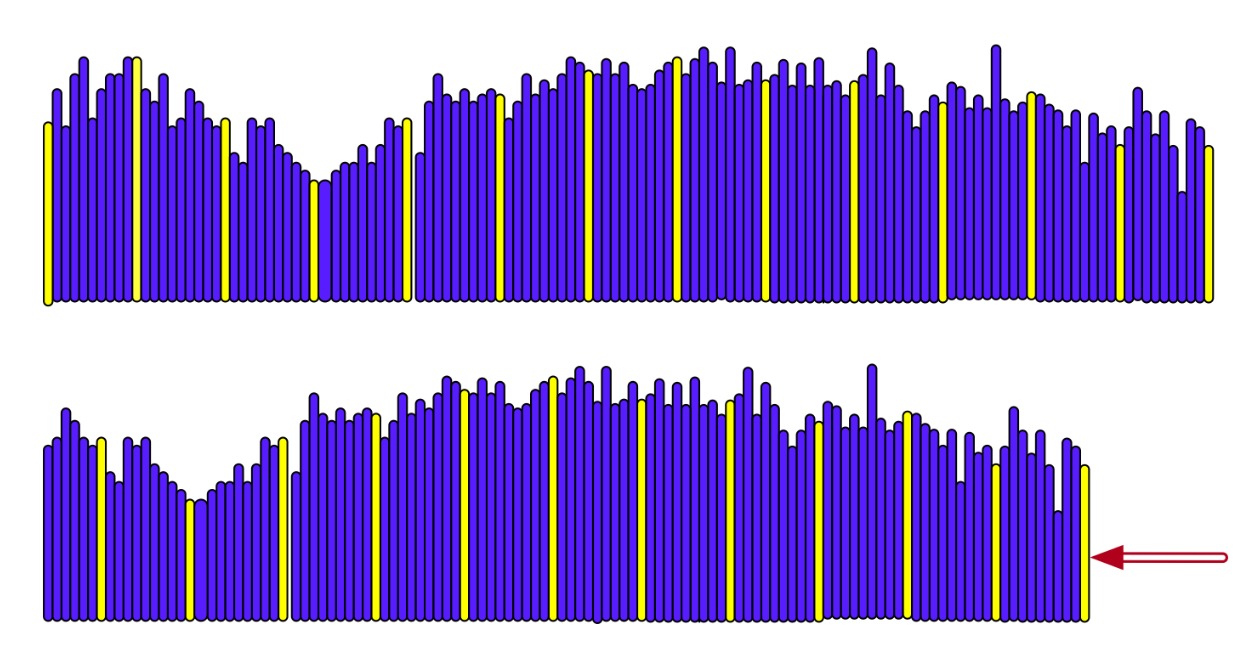
\includegraphics[width=\textwidth/2]{7.png}

shift the data by k and see how correlated it is with itself. highest peak represents
the most correlated point. tracing out the correlation as a vector. have to get 1 at lag = 0

\subsection{Autocorrelation:
Measure of correlation in time series
at different lags}

\begin{itemize}
  \item What is the value at lag t = 0?
  \item What does a peak at t = 7 mean?
\end{itemize}

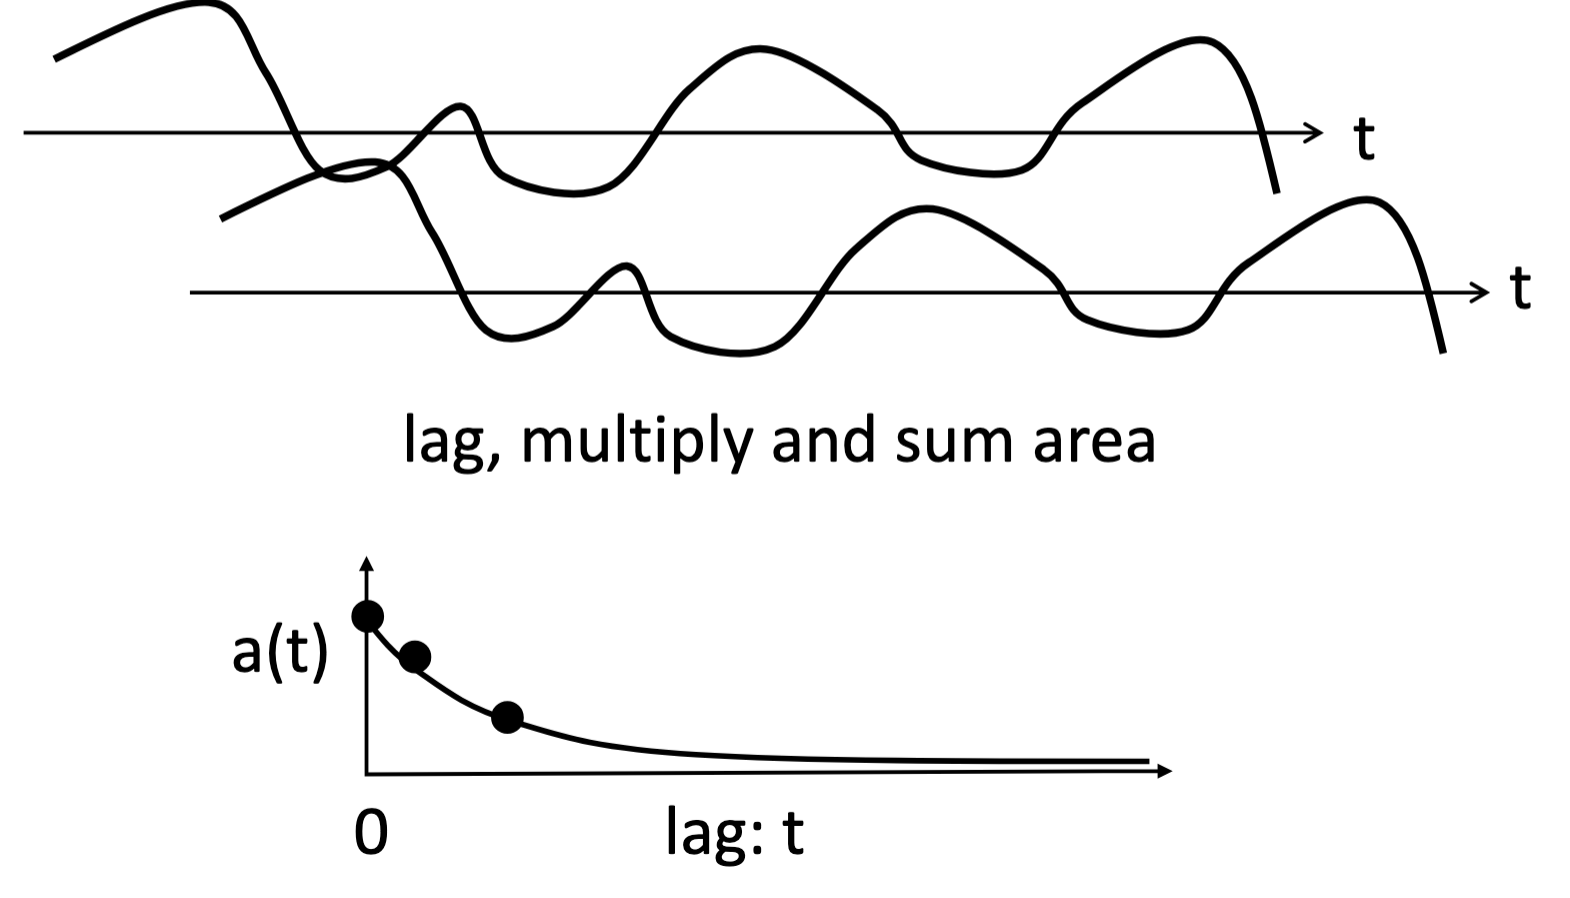
\includegraphics[width=\textwidth/2]{8.png}

\subsection{Autocorrelation Example}
Autocorrelation for
Chenai temperatures

\begin{itemize}
  \item High auto-correlation
  for the next day and
  for a year afterwards
  \item The light blue
  denotes significance
\end{itemize}

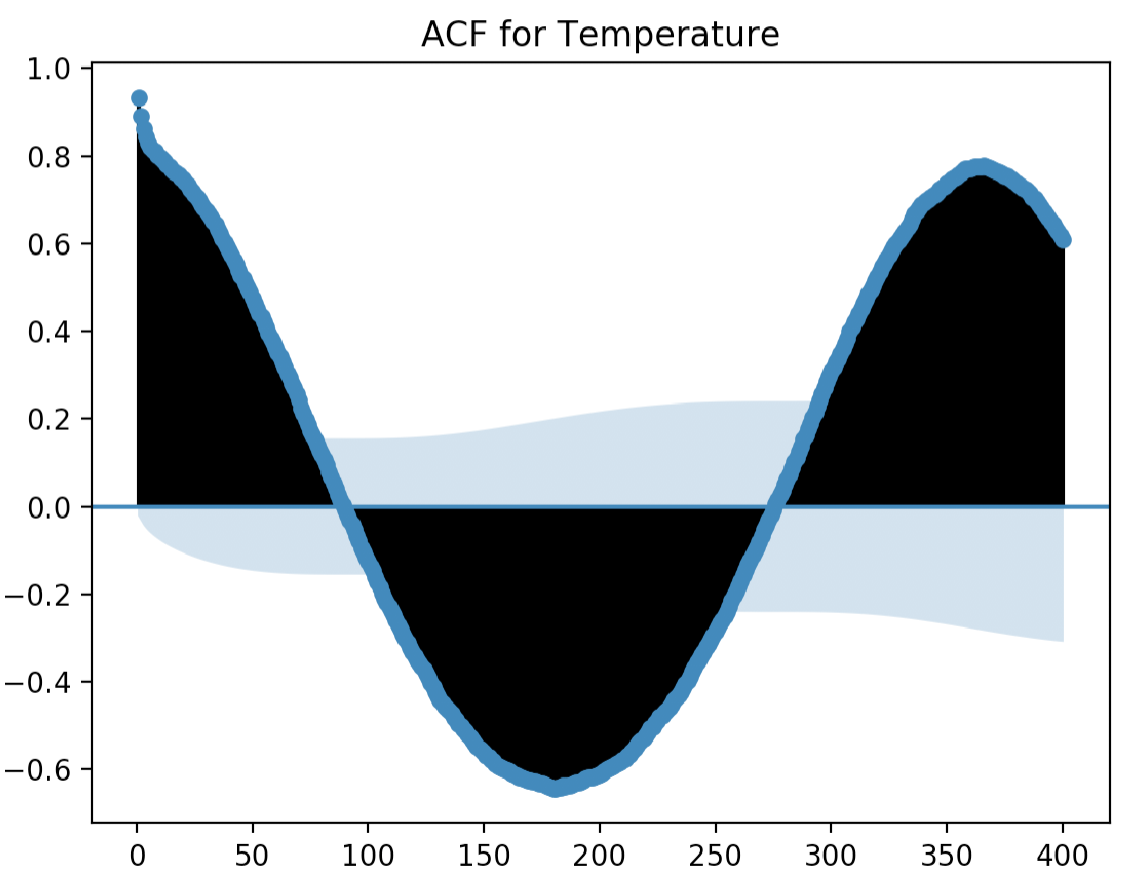
\includegraphics[width=\textwidth/2]{9.png}
\begin{verbatim}
  daily measurements. negative correlation with the seasonal changes. 
  there is autocorrelation
  in the air temperature. lag: t.
\end{verbatim}

\subsection{Cross-correlation}
\begin{itemize}
  \item Consider how one time
  series “predicts another”
  \begin{itemize}
    \item Example: how does the
    amount of rainfall affect
    (predict) the discharge water
    flow rate of a river measured
    at a given point?
    \begin{itemize}
      \item Discharge correlated with rain
      \item Discharge is delayed behind
      rain because rain takes time
      to drain from the land
    \end{itemize}
   \item  Compute Pearson
   correlation of one time
   series shifted by a lag of t
   time steps vs. the other
  \end{itemize}
\end{itemize}

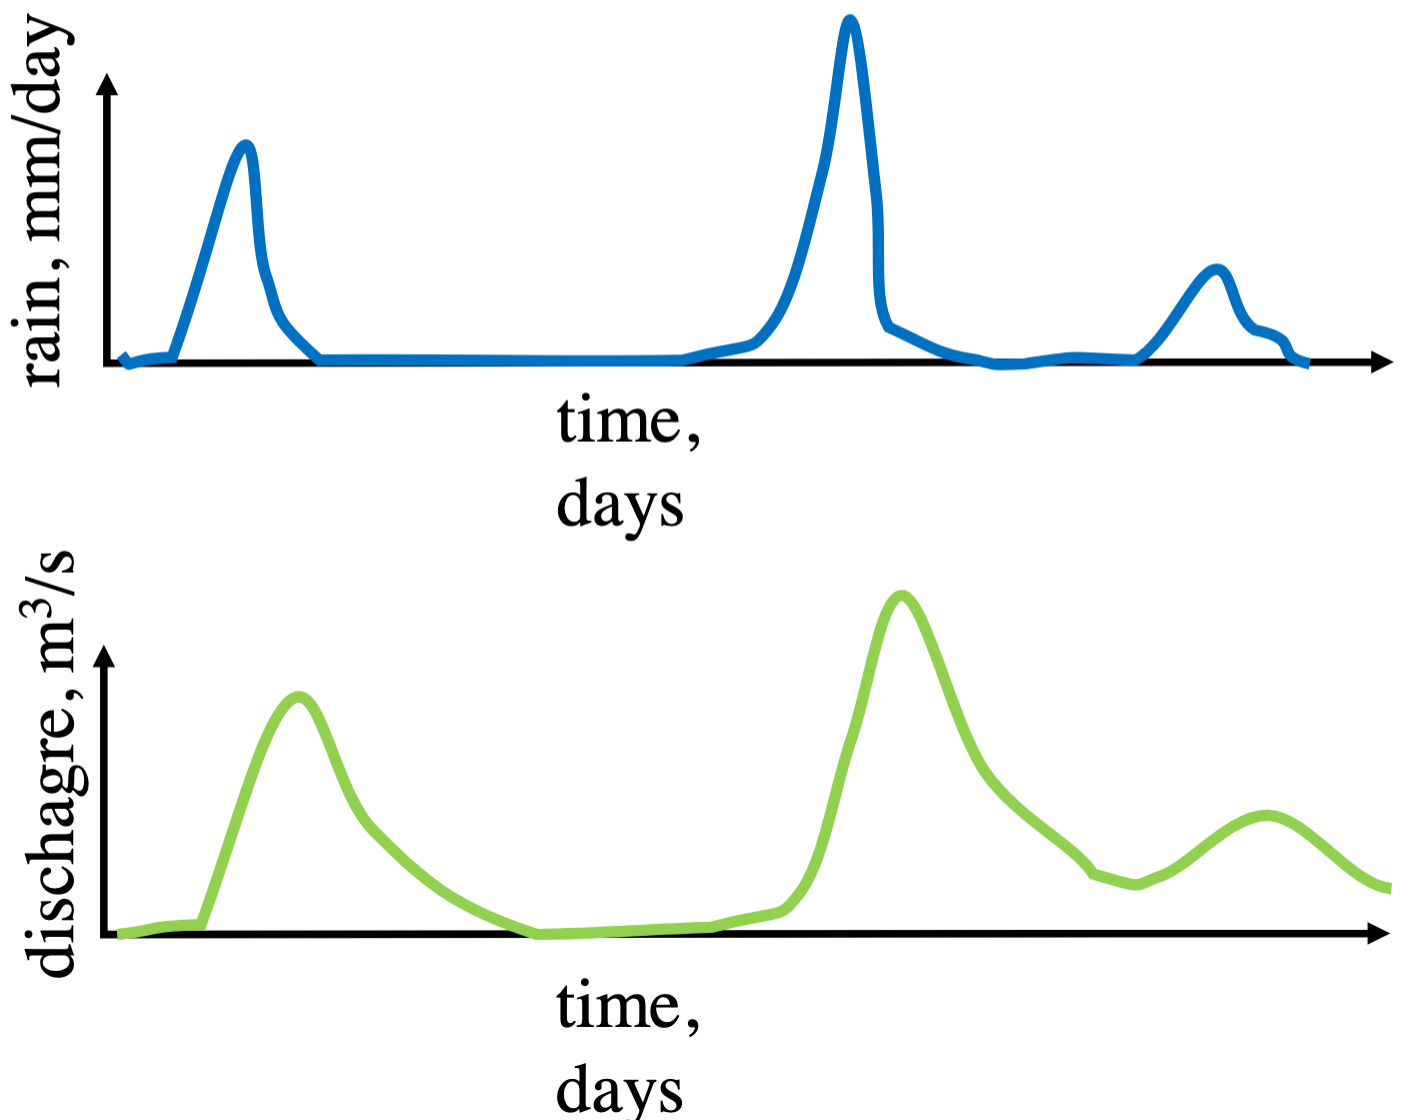
\includegraphics[width=\textwidth/2]{10.png}

\begin{verbatim}
  takes time for water to flow. 
  the peak of the discharge is delayed behind the peak of the rain.
\end{verbatim}

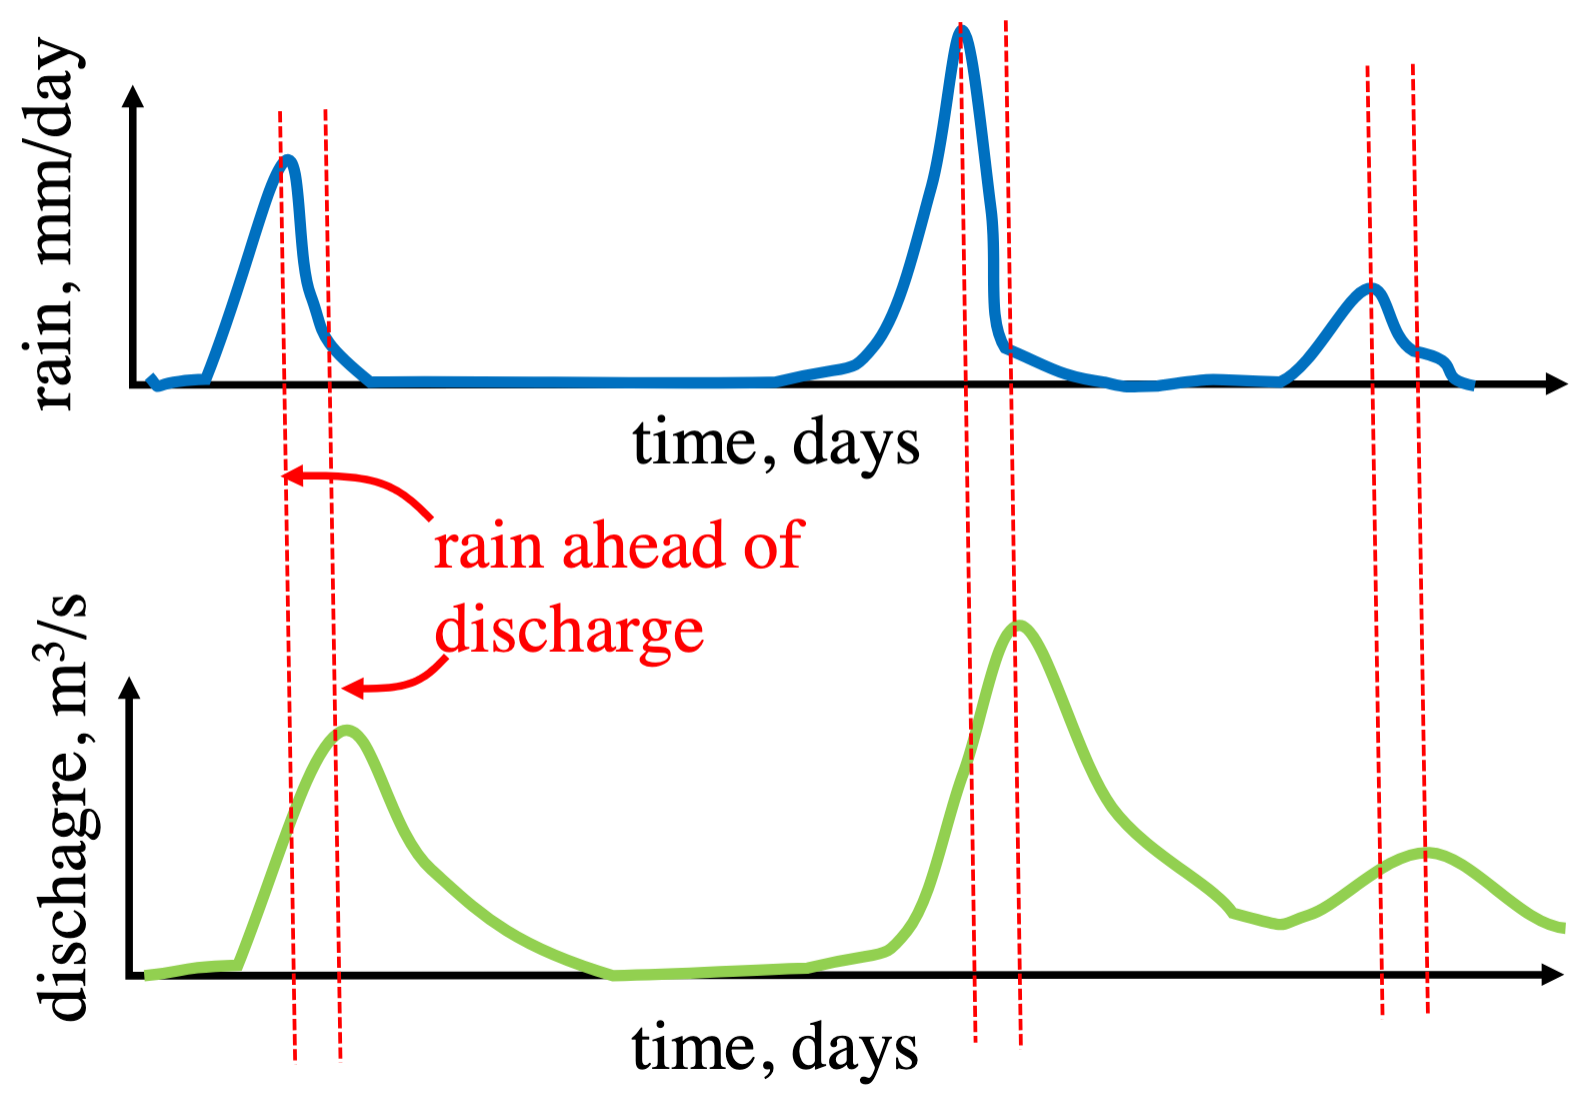
\includegraphics[width=\textwidth/4]{11.png}
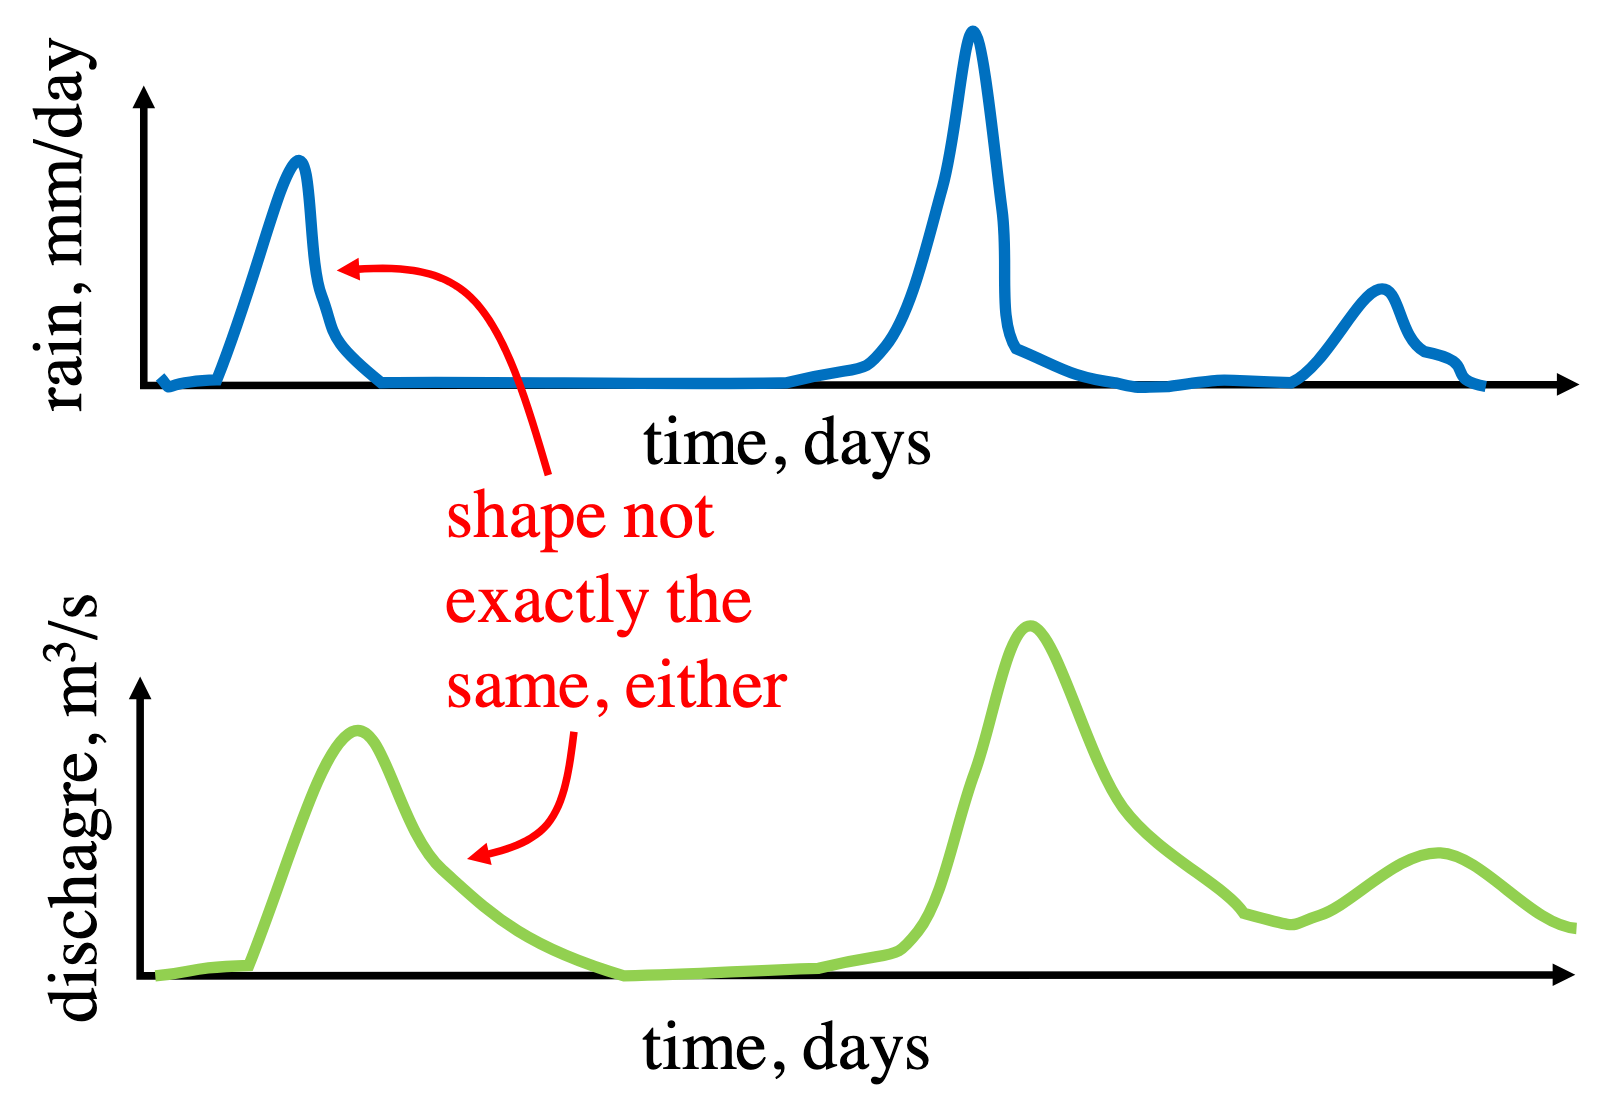
\includegraphics[width=\textwidth/4]{12.png}

\begin{note}
  how do we find the lag automatically? 
  shift at which the correlation peaks is the lag.
\end{note}

\subsection{Cross-correlation
Measure of correlation between two time series
at different lags}
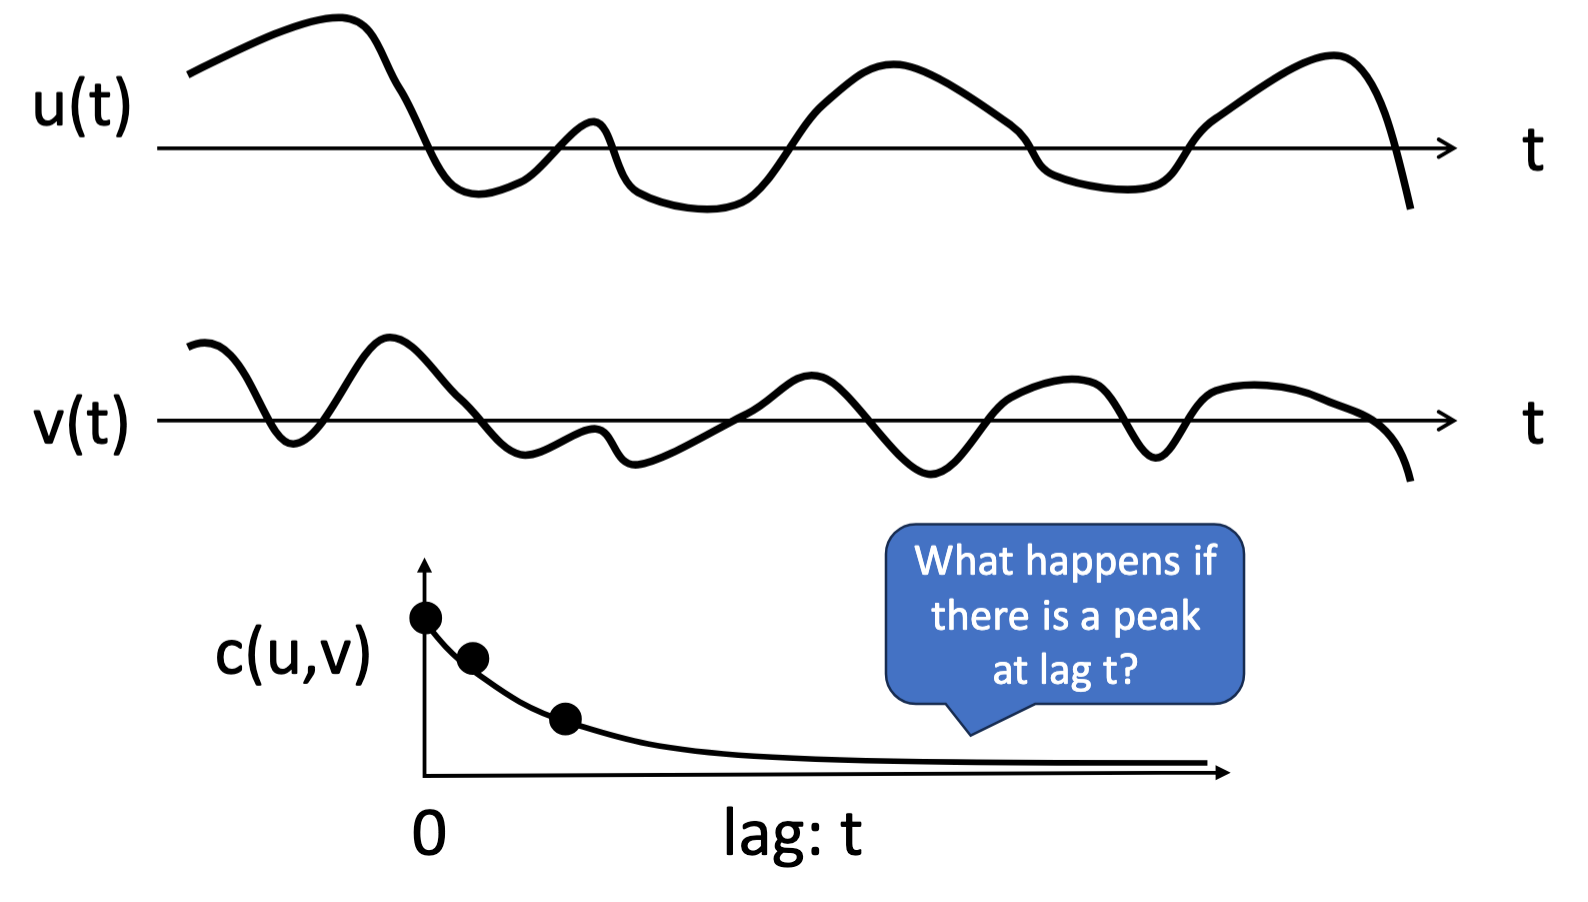
\includegraphics[width=\textwidth/2]{13.png}

\begin{note}
  the cross-correlation does not necessarily peak at 0. the peak is the lag at which the two series are most correlated.
\end{note}

\section{Smoothing}
\subsection{Smoothing}
\begin{itemize}
  \item Given a complete (noisy) dataset, what can I infer about the
  true state of nature in the past?
  \item Given a noisily measured signal, can I reconstruct the true
  signal from the data?
  \item Now that my spacecraft has flown around the moon, what the
  distance of its closest approach to the moon?
\end{itemize}

\subsection{Smoothing
(example of 3-point weighted average smoothing)}
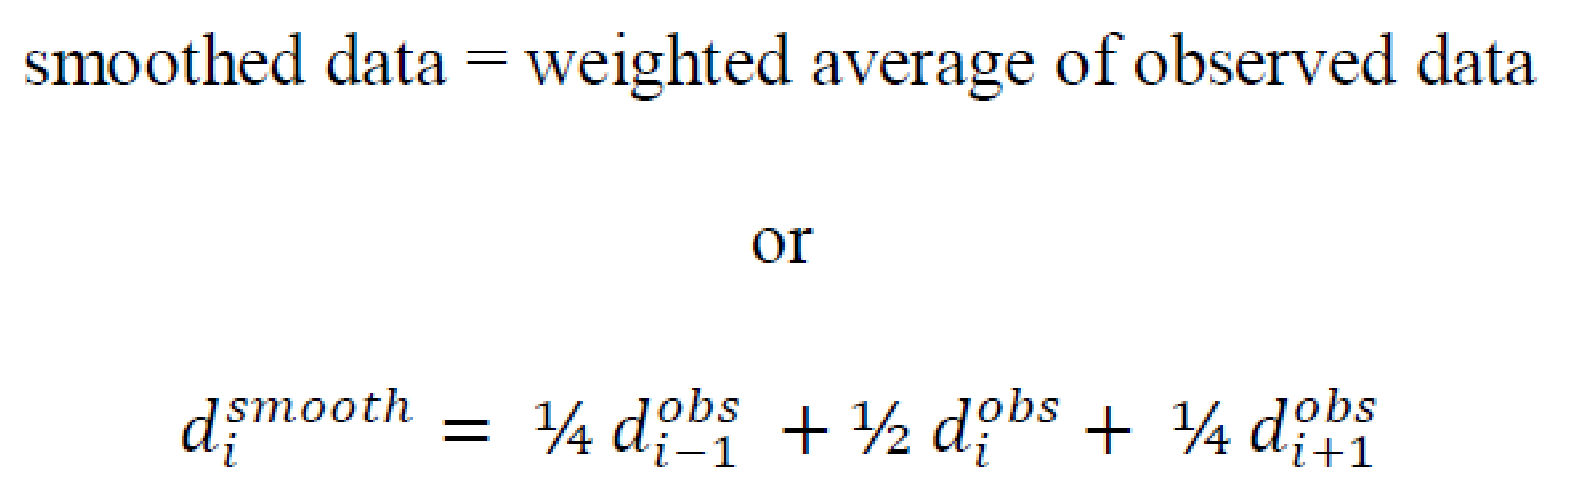
\includegraphics[width = \textwidth/2]{14.png}

i is the index of the data point, and t is the time index.

\subsection{Non-causal Smoothing}
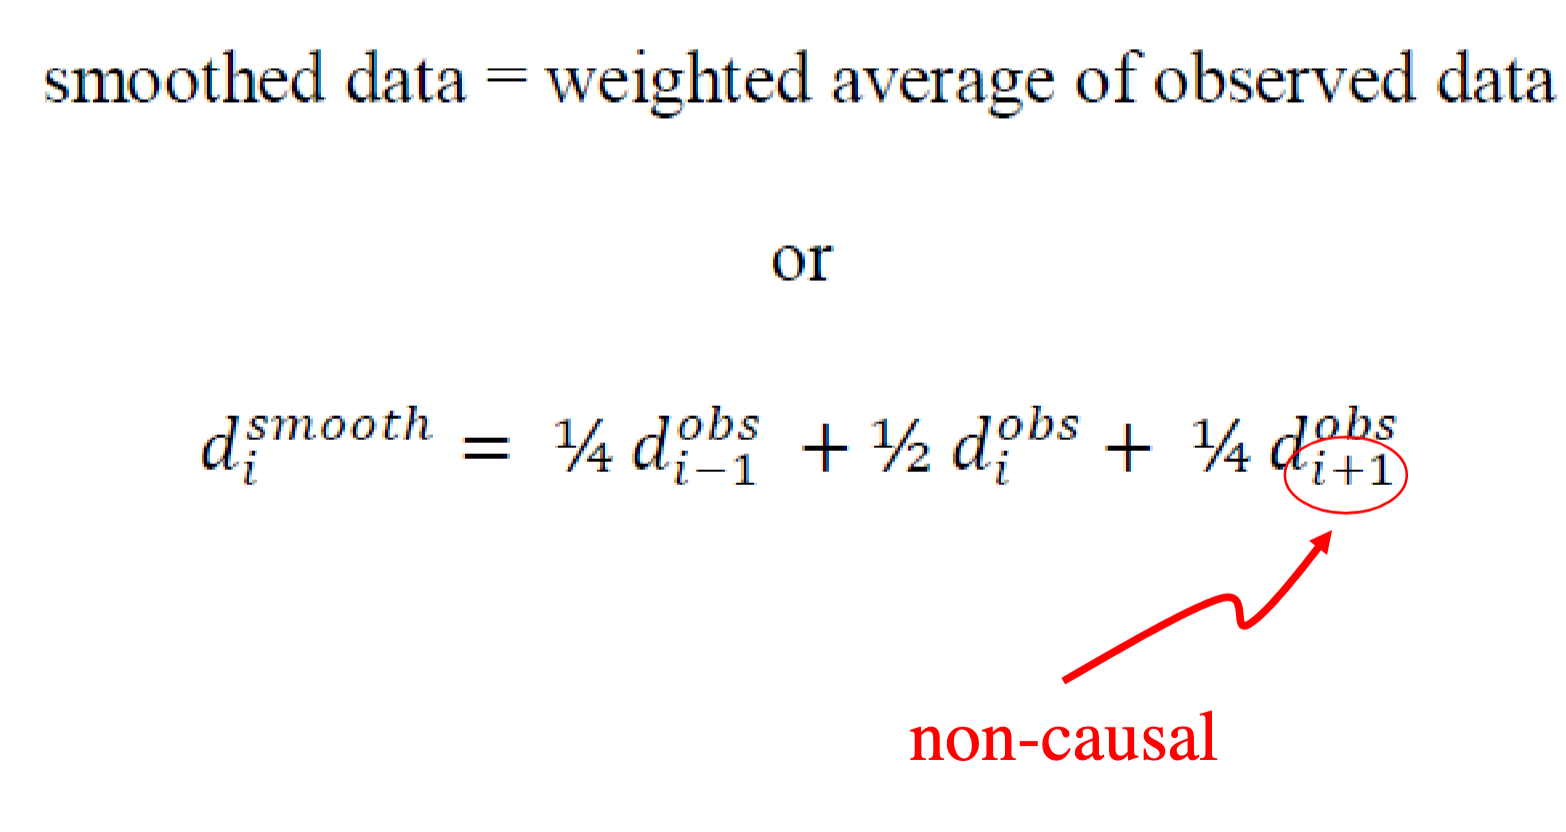
\includegraphics[width = \textwidth/2]{15.png}

you cannot use this form of smoothing for forecasting. the smoothed value depends on future values. causal smoothing is used for forecasting. causal smoothing is used for filtering and forecasting. non-causal smoothing is used for smoothing. causal smoothing is used for filtering and forecasting. 

non-causal is using data from the future to predict the past

filtering and forecasting not tested

\subsection{Causal Smoothing
(smoothed value does not depend on future)}
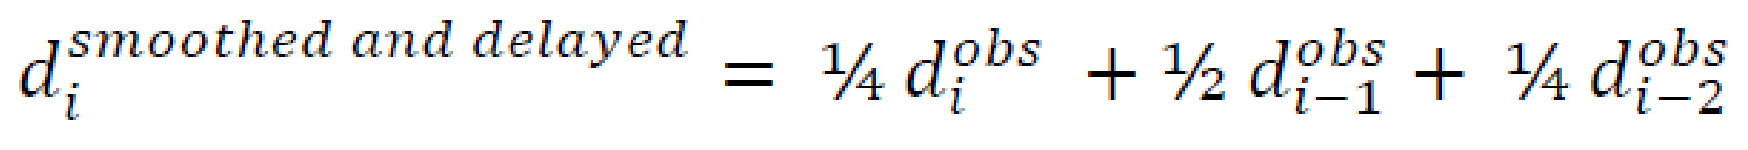
\includegraphics[width = \textwidth/2]{16.png}

only use lagged values to predict the current value.

\subsection{Triangular-weighted Smoothing Filters}
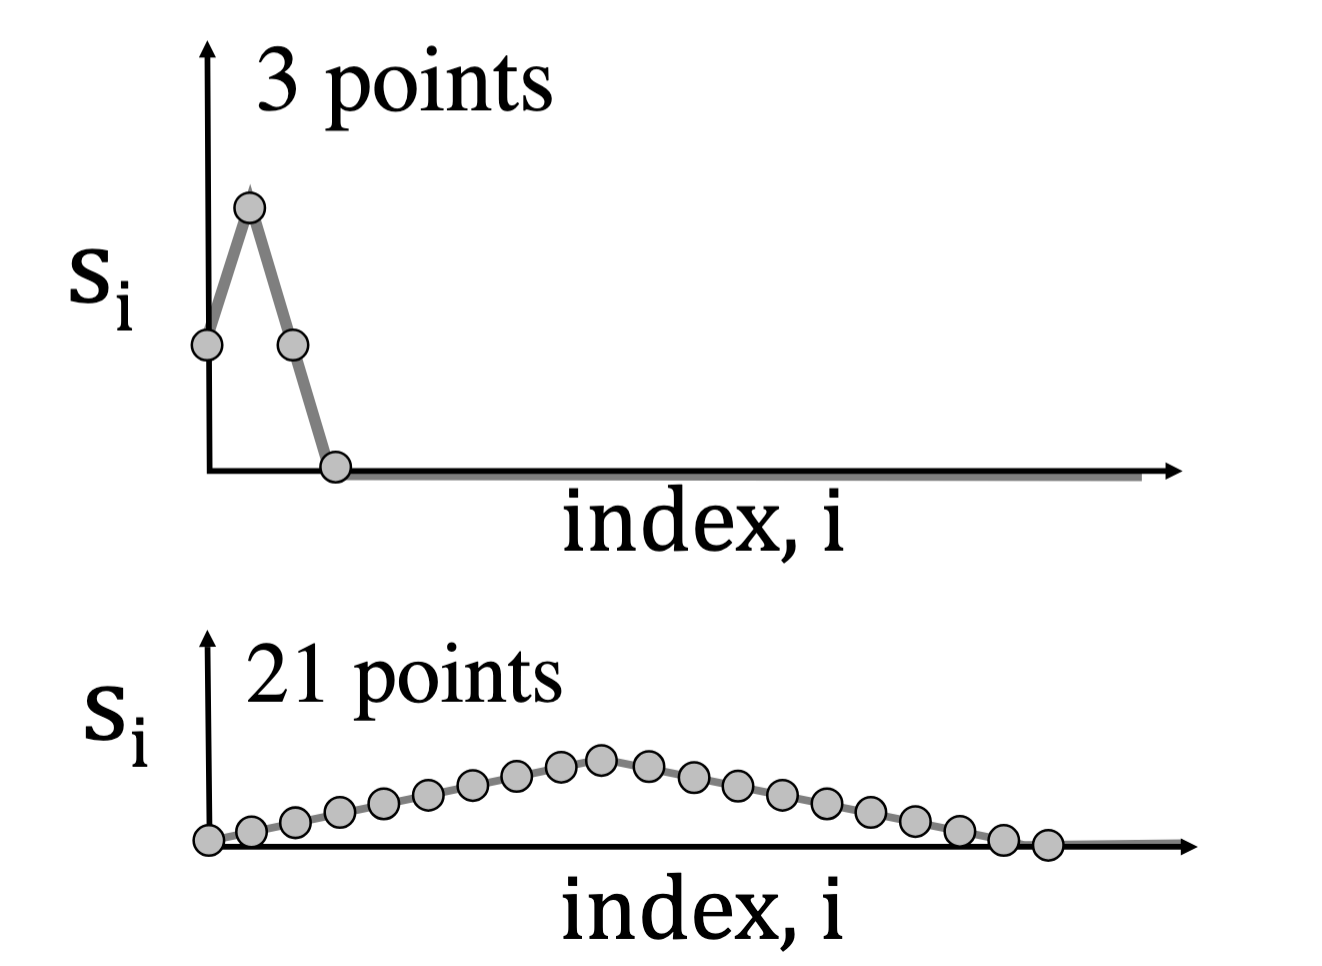
\includegraphics[width = \textwidth/2]{17.png}

the weights form a triangle. the weights are highest at the center and decrease as you move away from the center.

\subsection{Smoothing of Neuse River Hydrograph}
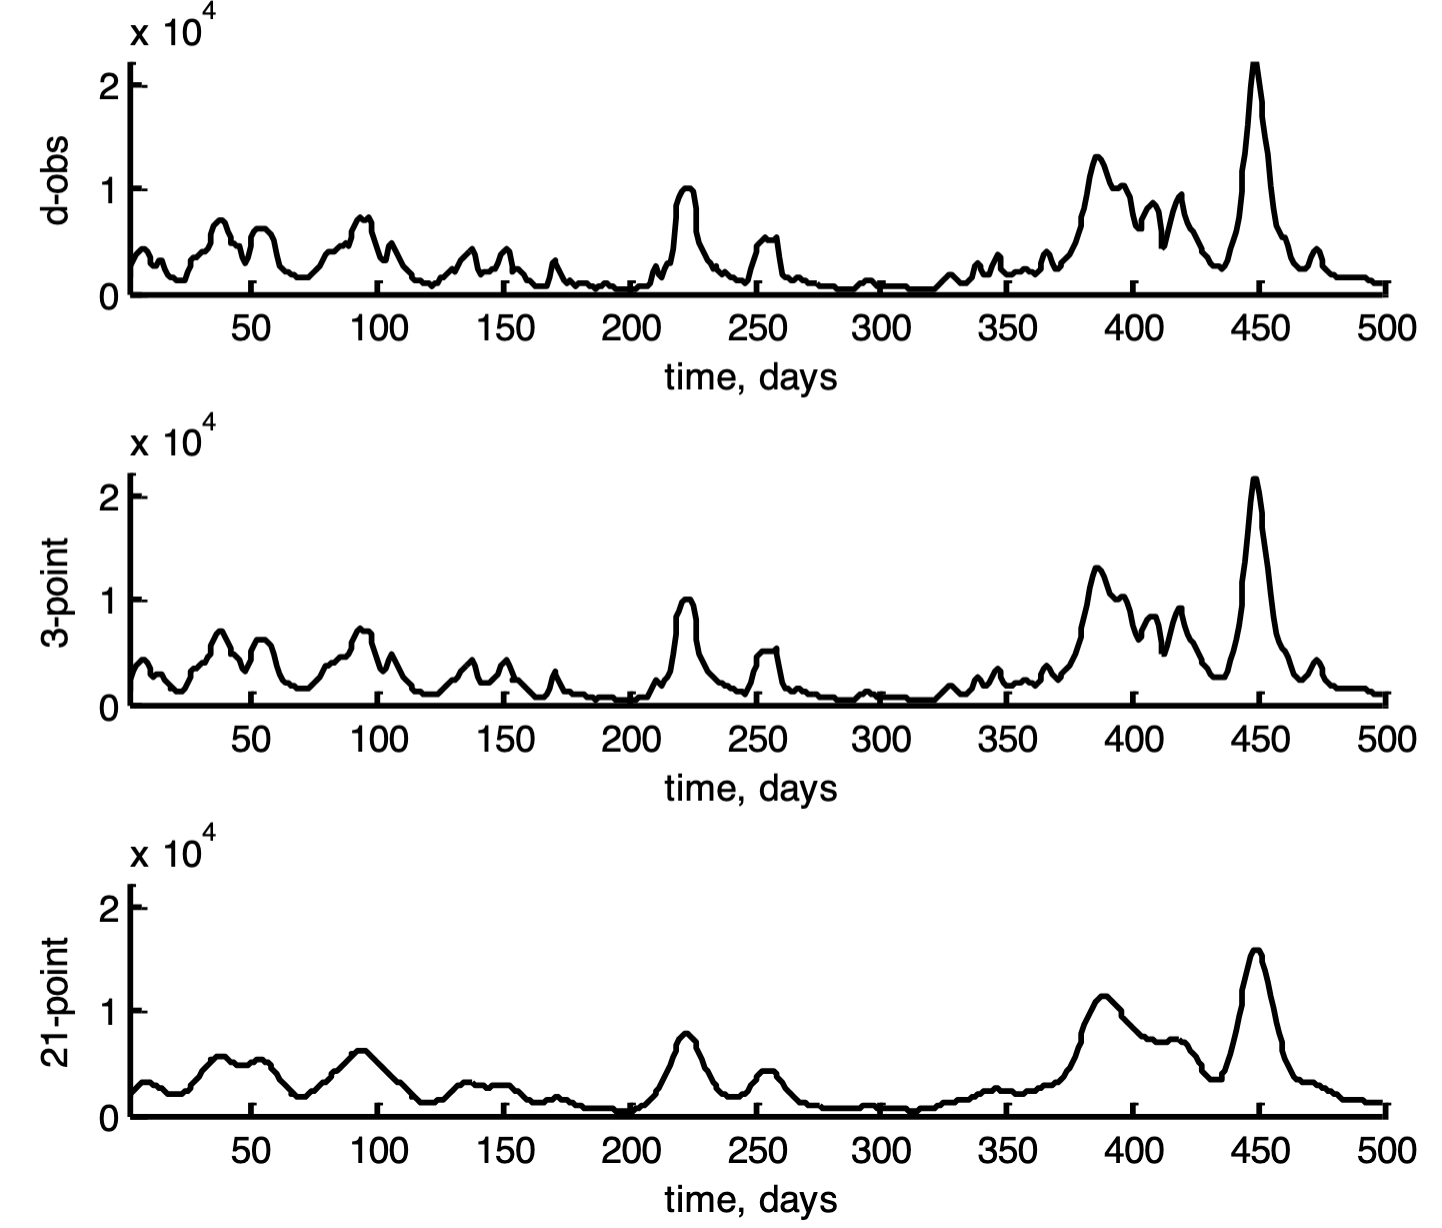
\includegraphics[width = \textwidth/2]{18.png}

\subsection{Smoothing Methods}
\begin{itemize}
  \item Box (windowed average) smoothing
  \begin{itemize}
    \item Uniform weights within a fixed window size
  \end{itemize}
  \item Triangular-weighted and Gaussian smoothing (make it normal)
  \begin{itemize}
    \item See previous slide for triangular weighting
    \item Gaussian just uses Gaussian-shaped weights
  \end{itemize} 
  \item Exponential smoothing
  \begin{itemize}
    \item Exponential decay to weights, efficiently computed over all history
    \item compute the next time point prediction as the observed timepoint + (1-alpha) * previous prediction
  \end{itemize}
\end{itemize}
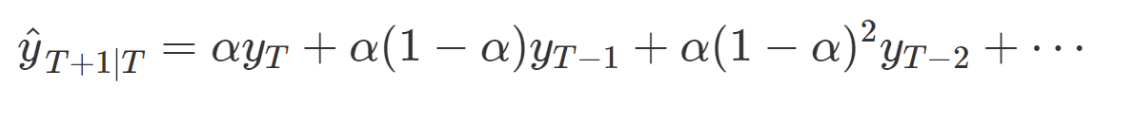
\includegraphics[width = \textwidth/2]{19.png}

s1 = alpha * x1 + (1-alpha) * s0 = x0

s2 = alpha * x2 + (1-alpha) * alpha * x1 + $(1-alpha)^2$ * s0 


ARIMA (not covered) - An autoregressive (trained) predictive regression model

\end{document}